\documentclass[10pt]{article}
\usepackage{multicol}
\usepackage{graphicx}
\usepackage{parskip} % For adding small vspace between 
                    %the paragraphs and not introducing
                    % any indentation
\usepackage{booktabs} % for better tables
\usepackage{siunitx}  % for units formatting
\usepackage{tabularx}
\usepackage{amsmath,amssymb, amstext}
\pagestyle{plain}

% preamble
\title{3D Mouse Documentation}
\author{Aniruddho}
\date{Last Updated: \today}


\begin{document}

\maketitle           % This one makes the titles



\section*{Abstract} % This one is single column

{\itshape This project presents the design and implementation of a low-cost 3D  
mouse using an MPU6050 inertial measurement unit (IMU) and an ESP32 microcontroller 
with Bluetooth Low Energy (BLE) connectivity. The device is developed as a motion-based 
human-computer interface capable of replacing or complementing conventional input 
peripherals. Raw accelerometer and gyroscope data are fused using a lightweight 
complementary filter, with bias correction methods applied to reduce drift and 
enhance stability. The processed motion data is mapped to standard Human Interface 
Device (HID) reports, enabling wireless cursor control and button interactions on 
a host computer without additional drivers. Performance metrics considered include 
latency, drift stability, sensitivity, and responsiveness, with emphasis on optimizing 
sensor calibration, real-time filtering, and BLE transmission rate. The prototype 
demonstrates the feasibility of developing an affordable, open-source alternative 
to commercial 3D input devices, highlighting both its practical usability and 
potential for extension into gaming, virtual reality, and advanced human-machine 
interaction research.}








\section*{Introduction} % This one will be 2 column
The evolution of human-computer interaction (HCI) has increasingly emphasized 
devices capable of capturing three-dimensional (3D) motion, enabling more 
intuitive and precise control in applications such as computer-aided design, 
gaming, and virtual reality. Conventional input peripherals, such as standard 
mice and trackpads, are limited to two degrees of freedom and often require 
complex mappings for 3D navigation. To address this limitation, dedicated 3D 
mice have been developed; however, these devices are typically expensive and 
proprietary, limiting accessibility for research and hobbyist development.
This project proposes the design and implementation of a low-cost, wireless 3D 
mouse using an MPU6050 inertial measurement unit (IMU) and an ESP32 
microcontroller with Bluetooth Low Energy (BLE) connectivity. The device captures 
hand motion along multiple axes, processes orientation and displacement data in 
real time, and transmits HID-compliant reports to a host computer. The system 
aims to provide an open-source alternative that replicates the fundamental 
functionality of commercial 3D mice while remaining accessible for 
experimentation, customization, and educational purposes. The objectives of this 
work are threefold: (1) to develop a robust, drift-stabilized motion sensing 
system using low-cost MEMS sensors, (2) to implement a wireless BLE HID interface 
for seamless host integration, and (3) to evaluate the device in terms of latency, sensitivity, and responsiveness. This project establishes a foundational platform for further enhancements, including advanced sensor fusion, gesture recognition, and extended control capabilities, offering a practical contribution to accessible HCI research.










\section*{System Design}


The proposed 3D mouse system is designed as a compact motion-sensing human-computer interface. The hardware consists primarily of two components: an MPU6050 inertial measurement unit (IMU) and an ESP32 microcontroller. The MPU6050 integrates a tri-axial accelerometer and gyroscope, providing six degrees of freedom (6-DoF) motion data. The ESP32, equipped with native Bluetooth Low Energy (BLE) capability, serves both as the data-processing unit and as the communication interface to the host device. The MPU6050 communicates with the ESP32 via the I²C protocol, ensuring efficient acquisition of real-time motion data. The ESP32 processes this data and formats it according to the Bluetooth Human Interface Device (HID) specification, thereby emulating a standard mouse. This design eliminates the need for additional drivers on the host system, offering seamless integration across operating platforms. A minimal set of push-buttons is also incorporated to provide left- and right-click functionality, thus replicating the essential features of a conventional mouse.



\section*{Methodology}

The development methodology was divided into three key stages: sensor data acquisition, signal processing, and HID report generation.

\textbf{Sensor Data Acquisition:}
The MPU6050 inertial measurement unit provides raw accelerometer and gyroscope 
readings at defined sampling rates. These outputs were calibrated to remove 
sensor bias and scaled to physical units. For this study, the accelerometer was 
sampled at 1 kHz, while the gyroscope was sampled at its maximum supported rate 
of 8 kHz. The acquired data formed the basis for subsequent filtering and motion 
estimation.

\textbf{Signal Processing:}
Raw sensor readings are inherently noisy and prone to drift. To mitigate these 
issues, a complementary filter was implemented to fuse gyroscope and accelerometer 
data, yielding stable orientation estimates. Drift stabilization techniques, 
including bias compensation, were incorporated to reduce cumulative integration 
error. The processing pipeline first acquired raw samples at 1 kHz, which were 
averaged over an interval determined through Allan variance analysis to suppress 
high-frequency noise. Stochastic Calibration was then applied to correct sensor 
counts, followed by optional conversion to physical units. The processed values 
were truncated for stability and mapped to cursor pixel displacements before 
being transmitted as control commands. This stage ensured that IMU-derived 
orientation and motion data were both stable and responsive.

\textbf{HID Report Generation and Transmission:}
The processed orientation and motion values were mapped into displacement 
commands along the X and Y axes. The ESP32 microcontroller encoded this 
information into HID-compliant reports, which were transmitted over Bluetooth 
Low Energy (BLE) to the host device at fixed intervals. Button press events were 
also incorporated into the HID reports, enabling standard mouse functionality. 
This methodology emphasized low latency, noise suppression, and BLE connection 
stability, which are critical for practical 3D input device performance.




\section*{Implementation}

The implementation phase comprised both hardware integration and firmware 
development, followed by preliminary validation of the prototype system.

\subsection*{Hardware Integration}
The MPU6050 was interfaced with the ESP32 microcontroller via the I²C protocol, 
with pull-up resistors on the SDA and SCL lines to ensure reliable communication. 
Two push-buttons were connected to general-purpose input/output (GPIO) pins 
configured with internal pull-up resistors, enabling left- and right-click 
inputs. Power was supplied through a USB interface, with an optional battery 
connection provided to support portable operation.

\subsection*{Firmware Development}
The firmware was developed in C++ using the Arduino framework. During system 
initialization, the MPU6050 was configured and continuously polled for motion 
data. Calibration routines were implemented at startup to correct sensor bias 
offsets. A complementary filter was executed in real time to estimate 
orientation, and a sensitivity scaling factor was incorporated to adjust cursor 
responsiveness.  
For communication, the ESP32 was configured as a Bluetooth Low Energy (BLE) 
Human Interface Device (HID) using the \texttt{BLEHIDDevice} library. The HID 
report descriptor was customized to support two motion axes and three mouse 
buttons, allowing the device to be recognized by the host system as a standard 
mouse without requiring additional drivers. Continuous HID notifications were 
transmitted at a fixed interval to provide smooth cursor updates.

\subsection*{Prototype Validation}
Initial validation confirmed reliable pairing between the prototype and a host 
computer, with functional cursor control achieved. The system demonstrated 
low-latency data transmission and basic usability, establishing a baseline for 
subsequent performance evaluation through numerical testing and experimental 
trials.





\section*{Error Modeling}

The implementation of theoretical concepts in real-world systems requires careful 
consideration of practical limitations, as no mathematical model can perfectly 
describe sensor behavior under all conditions. Various irregularities, such as 
manufacturing imperfections, temperature fluctuations, and electronic noise, 
introduce errors into the sensor readings. To adapt to these challenges, 
calibration and error modeling techniques were applied to characterize and 
mitigate these effects.

\subsubsection*{Stochastic Calibration (Allan Variance)}
Allan variance analysis was employed to characterize the stochastic error 
components of the inertial sensors. This method quantifies how measurement 
accuracy changes as data is averaged over different time intervals. At shorter 
averaging times, variance decreases due to the suppression of high-frequency 
noise. However, beyond a certain point, the variance begins to increase again as 
long-term bias drift dominates.  

For the present application, longer averaging times can be tolerated compared to 
higher-grade accelerometers, since the required bandwidth is limited to motions 
below 10 Hz. Thus, Allan variance provided a suitable framework to determine 
optimal averaging intervals for data acquisition and stability assessment.

Formally, for a time series $x_k$ sampled at intervals of $T_0$, the cluster 
size $m$ (number of samples per cluster) defines the averaging time $\tau = mT_0$. Let $M$ 
be the number of non-overlapping clusters, and $\bar{y}_i$ represent the mean of 
the $i$-th cluster. The Allan variance for averaging time $\tau$ is given by:

$$
\sigma^2(\tau) = \frac{1}{2(M-1)}\sum_{i=1}^{M-1}{(\bar{y}_{i+1} - \bar{y}_i)^2}
$$
\textbf{Gyroscope Allan Variance:}

\begin{center}
    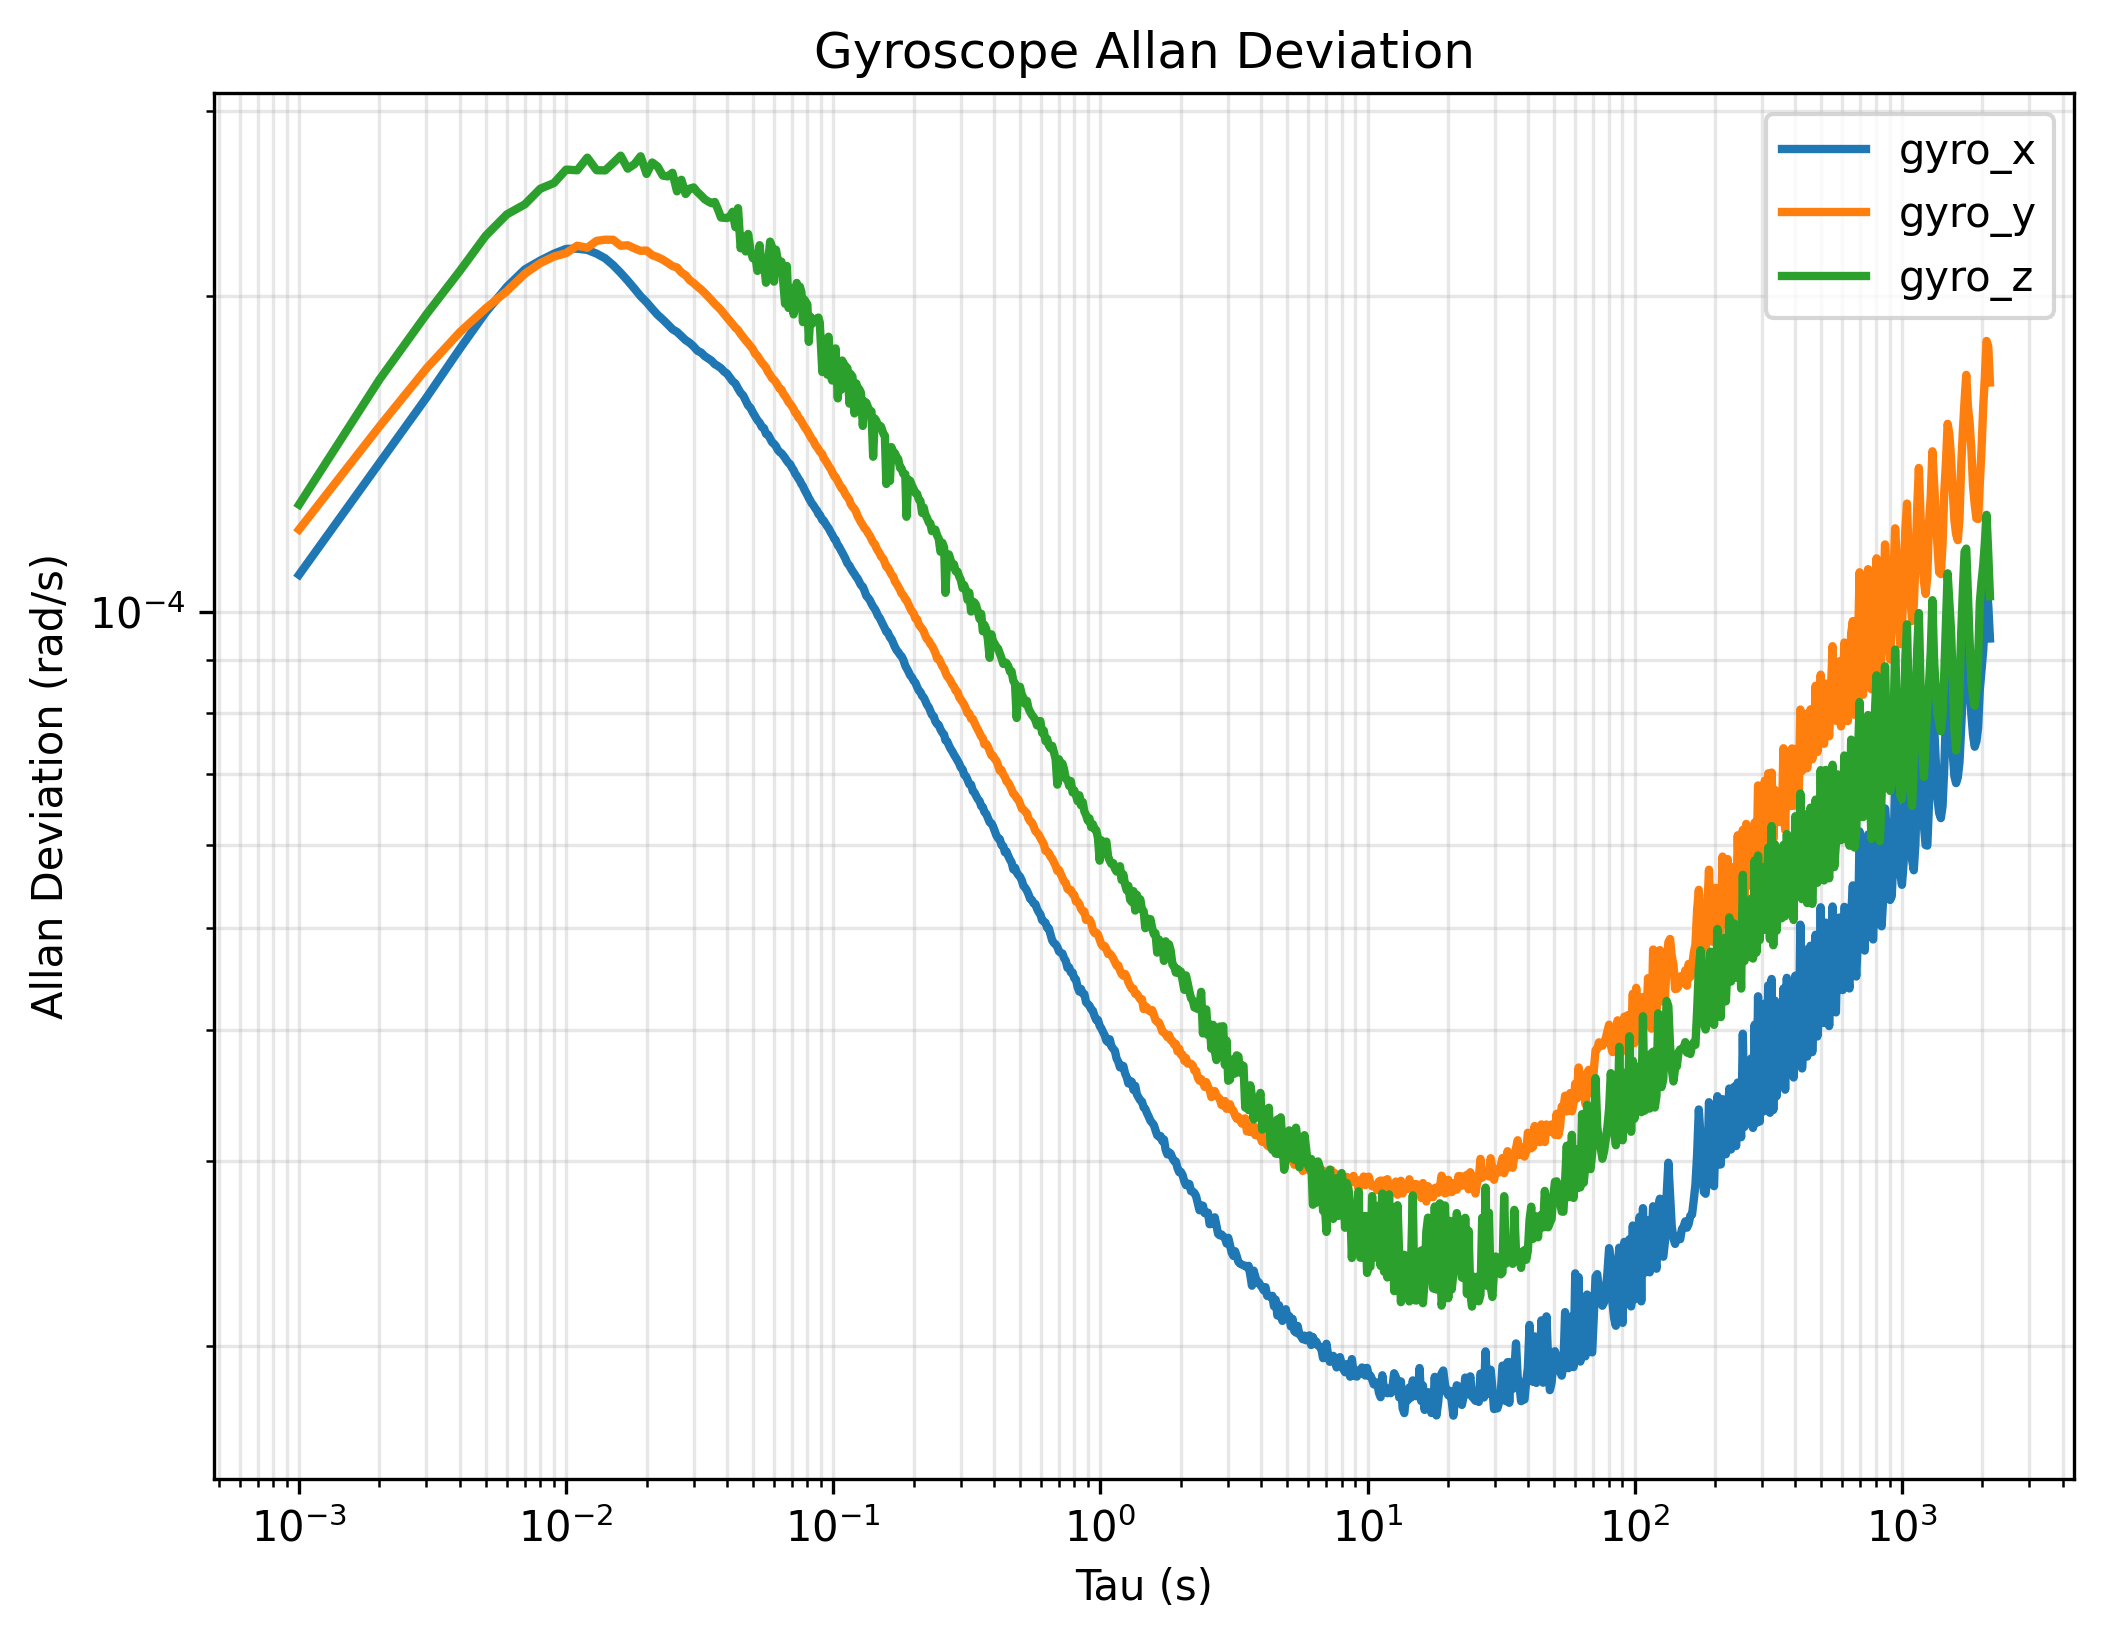
\includegraphics[width=12cm, height=10cm]{gyro_allan.png} % Placeholder for gyroscope plot
\end{center}

% ...
\begin{table}[h!]
    \centering
    \begin{tabularx}{\linewidth}{@{}l XXX@{}}
    \toprule
    \textbf{Parameter} & \textbf{X} & \textbf{Y} & \textbf{Z} \\
    \midrule
    ARW [$rad/s/\sqrt{Hz}$] & $3.428 \times 10^{-6}$ & $3.786 \times 10^{-6}$ & $3.999 \times 10^{-6}$ \\
    Bias Instability [rad/s] & $1.715 \times 10^{-5}$ & $2.743 \times 10^{-5}$ & $2.179 \times 10^{-5}$ \\
    Averaging Time [s] & 20.97 & 16.60 & 24.62 \\
    Bias Drift Onset [s] & $59.95$ & $61.72$ & $50.32$ \\
    \bottomrule
    \end{tabularx}
    \caption{Extracted Allan variance parameters for the gyroscope.}
\end{table}
    

\textbf{Accelerometer Allan Variance}


\begin{center}
    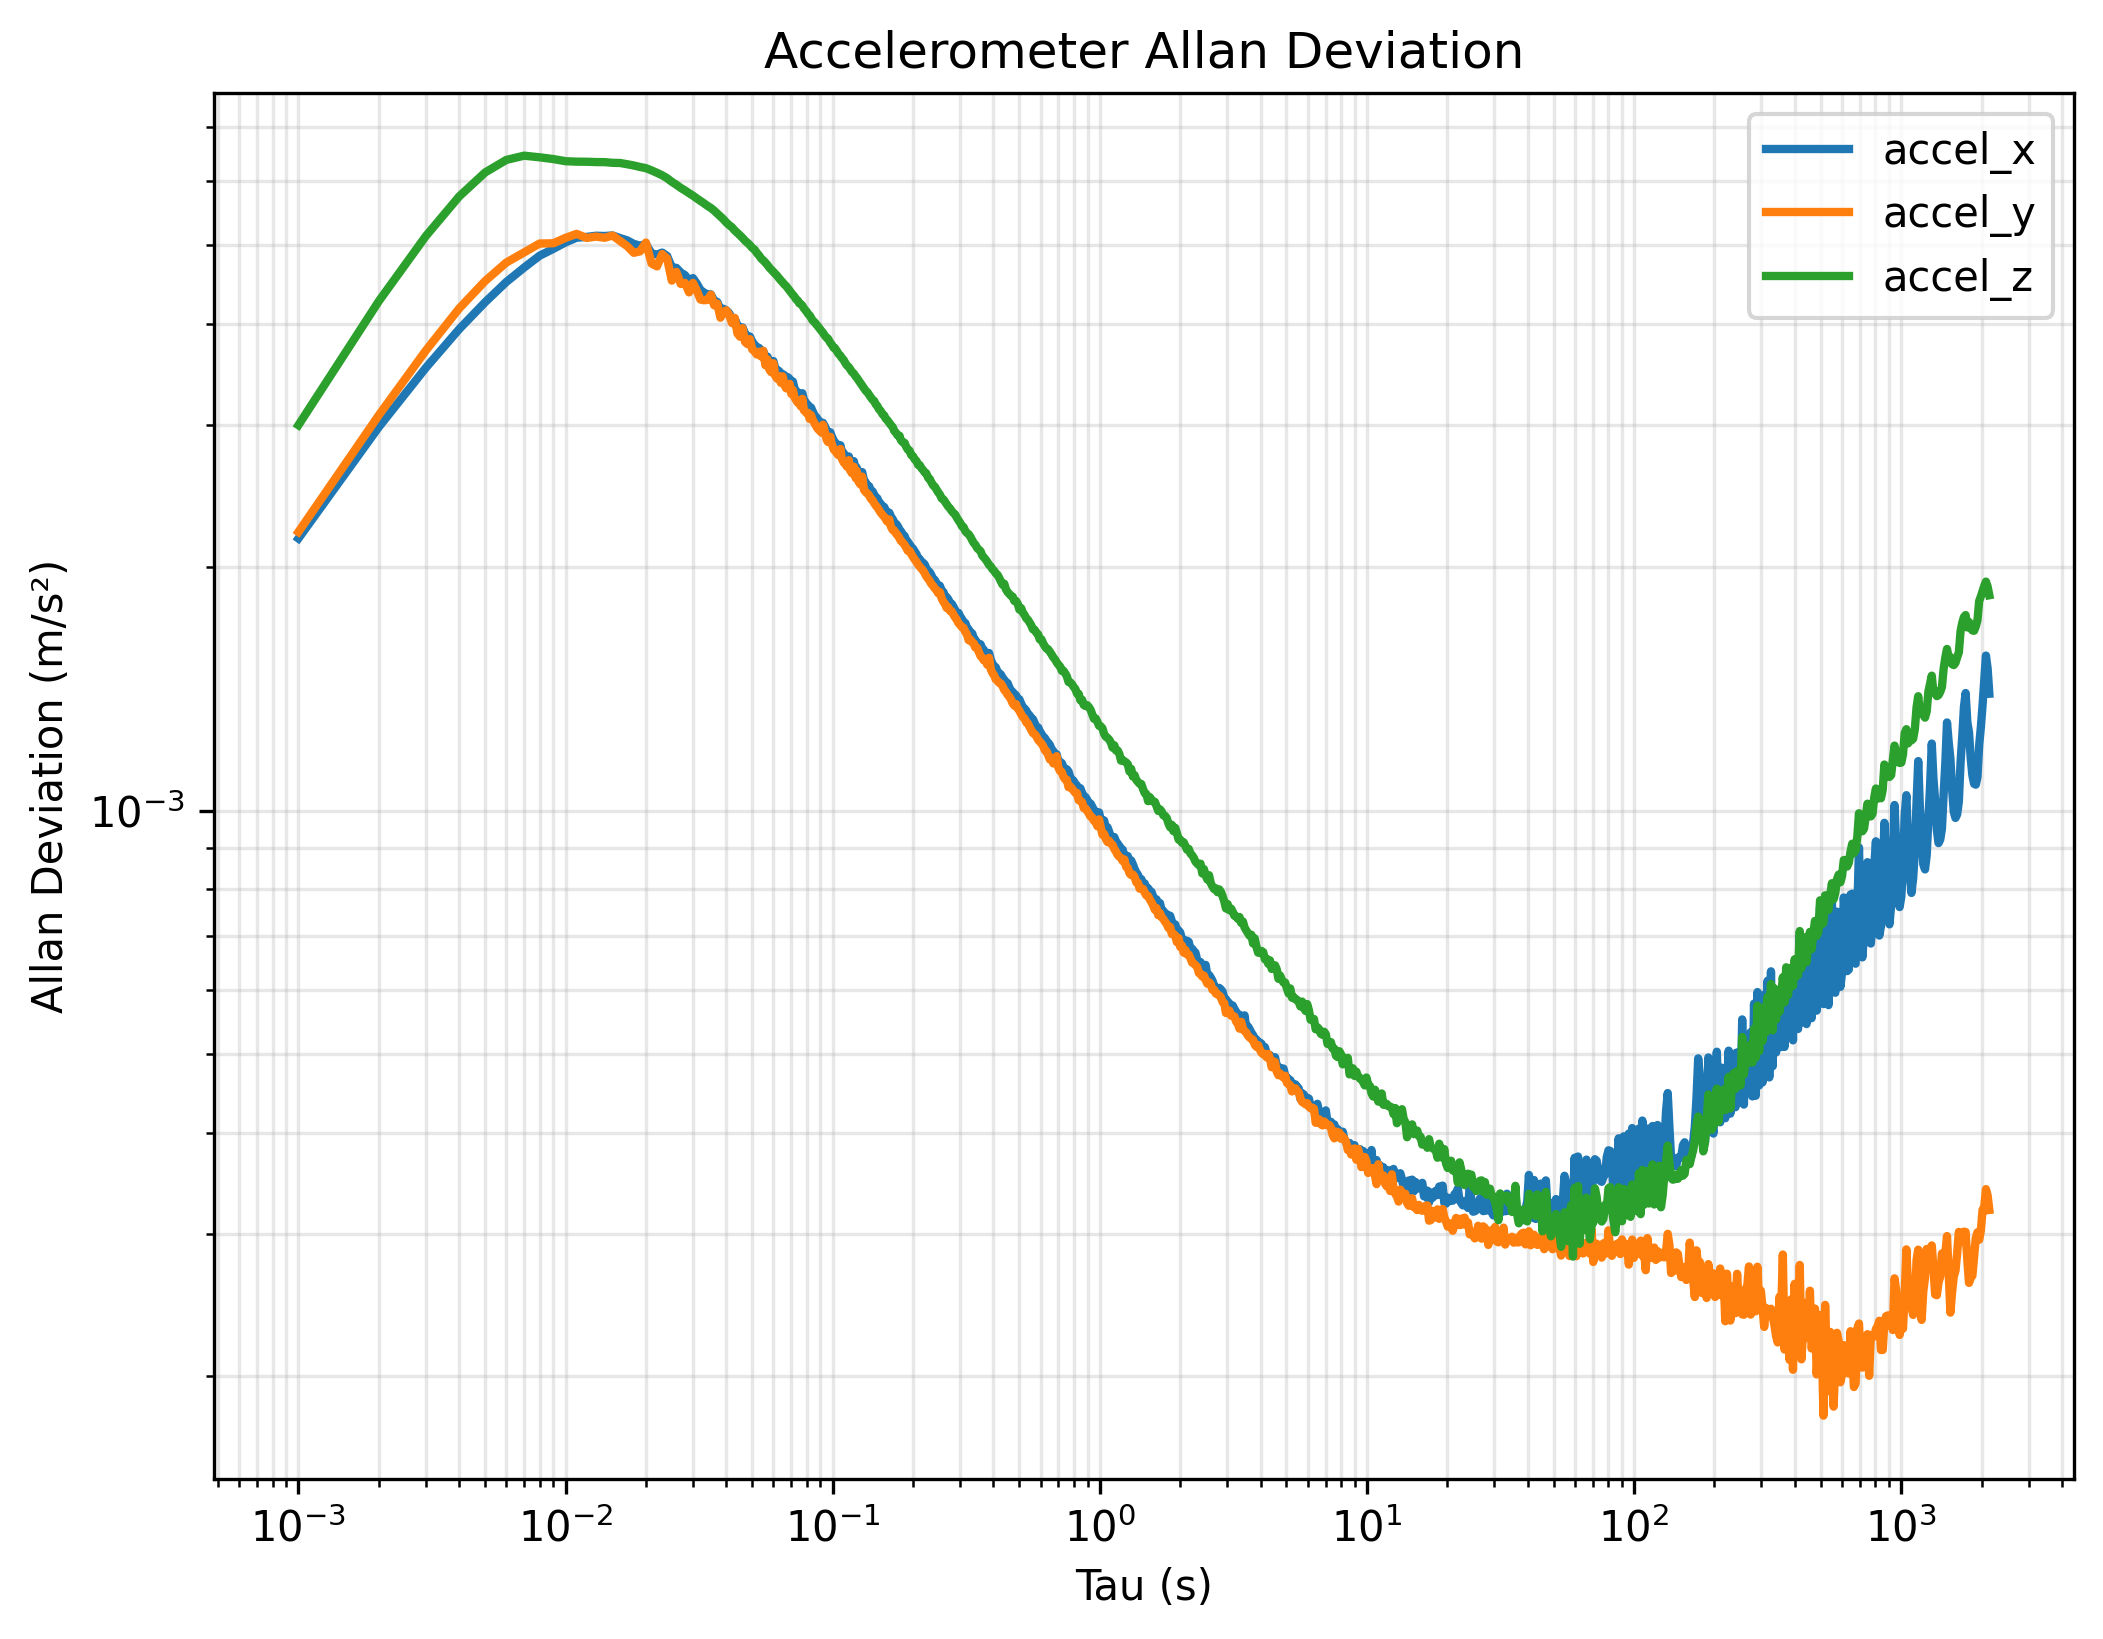
\includegraphics[width=12cm, height=10cm]{accel_allan.png} % Placeholder for gyroscope plot
\end{center}

% ...
\begin{table}[h!]
    \centering
    \begin{tabularx}{\linewidth}{@{}l XXX@{}}
    \toprule
    \textbf{Parameter} & \textbf{X} & \textbf{Y} & \textbf{Z} \\
    \midrule
    VRW [$m/s^2/\sqrt{Hz}$] & $6.861 \times 10^{-5}$ & $6.988 \times 10^{-5}$ & $9.472 \times 10^{-5}$ \\
    Bias Instability [$m/s^2$] & $3.044 \times 10^{-4}$ & $1.787 \times 10^{-4}$ & $2.810 \times 10^{-4}$ \\
    Averaging Time [s] &  48.87 & 511.98 & 59.08 \\
    Bias Drift Onset [s] & $95.62$ & $519.50$ & $131.81$ \\
    \bottomrule
    \end{tabularx}
    \caption{Extracted Allan variance parameters for the accelerometer.}
\end{table}




\subsection*{Deterministic Calibration}
\subsubsection*{Accelerometer 6 Point Calibration} Here we  find the 
$3\times3$ scale/misalignment matrix $M$ and a $3\times1$ matrix
$b$ such that:
$$
a_{True} = M(a_{raw} - b)
$$
where $a_{\text{true}}$ corresponds to the expected acceleration when the sensor 
is stationary and aligned with gravity. In this configuration 
(i.e., with the mouse body held stationary and oriented such that its sensitive 
axis is aligned with the gravitational vector), the accelerometer should ideally 
report a magnitude of $1g$. The six-point calibration procedure yielded the 
following calibration matrix $M$ and bias vector $b$:

$$
M = \begin{bmatrix}
    6.08997382\times10^{-5}  & 7.41227306\times10^{-7}    & 2.03088121\times10^{-6} \\
    1.69669384\times10^{-6}  & 6.12865742\times10^{-5}  & -1.71520618\times10^{-7}\\
    -3.16142589\times10^{-7} & 4.30764171\times10^{-6}  & 6.00314277\times10^{-5}
\end{bmatrix}
$$
$$
b = \begin{bmatrix}
    -0.05525702 & 0.01076481 & -0.03638963
\end{bmatrix}
$$
$$
bias_{gyro} = \begin{bmatrix}
        -0.05525702  & 0.01076481  & -0.03638963
\end{bmatrix}
$$
Following this calibration, additional fine-tuning will be applied to achieve 
sub-degree accuracy and improved stability.


\subsection*{Future Work}
Several improvements remain to be addressed in order to further enhance sensor 
performance. One key aspect is temperature compensation, which can mitigate 
thermal drift effects on both accelerometer and gyroscope measurements. 
In addition, gyro calibration can be performed during periods when the 
accelerometer indicates no motion, with consecutive gyro readings averaged over 
the optimal interval to establish an updated zero-rate reference.  

The deterministic calibration currently assumes a linear response that was used
in the calibration as ($a_{True} = M (a_{\text{raw}} - b)$), whereas in practice sensor 
behavior is often nonlinear. Future work should therefore focus on mapping 
the nonlinear sensor response to an equivalent linear model. Cross-axis 
alignment, another source of systematic error arising from manufacturing 
imperfections, should also be corrected to improve accuracy prior to the 
application of sensor fusion algorithms.  

It is noteworthy that many of these compensation and calibration techniques 
are already implemented internally in newer-generation IMUs such as the BMI160 
and ICM-426xx series from TDK/InvenSense. For applications requiring higher 
precision than the present prototype, these calibration steps can be performed 
with greater accuracy at the library or algorithmic level to meet specific 
performance requirements.






\section*{Discussion}

The calibration and error modeling results highlight the inherent limitations of 
the MPU6050 sensor package while also demonstrating the effectiveness of the 
applied corrections. The six-point deterministic calibration successfully reduced 
static bias and scale factor errors, producing a calibration matrix that aligned 
the accelerometer outputs with the expected 1~$g$ reference when stationary. 
This step was essential to establish a consistent baseline for orientation 
estimation.

The stochastic characterization using Allan variance provided further insight 
into the noise properties and drift behavior of the IMU. The gyroscope exhibited 
angle random walk (ARW) on the order of $10^{-6}$~rad/$\sqrt{s}$ and bias 
instability between $1.7\times10^{-5}$ and $2.7\times10^{-5}$~rad/s, 
with drift becoming dominant after approximately 50--60~s. The accelerometer 
demonstrated velocity random walk (VRW) values on the order of
$10^{-5}$~m/s$^2/\sqrt{Hz}$ and bias instabilities in the range of 
$1.8\times10^{-4}$ to $3.0\times10^{-4}~m/s^2$, with drift onsets between 95~s 
and 520~s depending on axis. These results confirm that while short-term noise 
can be effectively reduced through averaging, long-term drift remains a limiting 
factor for extended operation without external correction.

Together, these findings indicate that the prototype 3D mouse is suitable for 
short-term interactive tasks, where motions are constrained within tens of 
seconds, but less reliable for applications requiring long-duration stability. 
The behavior is consistent with expectations for an older consumer-grade IMU such 
as the MPU6050, which lacks built-in temperature compensation and advanced 
calibration features found in newer devices. Nonetheless, the calibration 
framework and Allan variance analysis provide a valuable foundation for improving 
performance through sensor fusion, periodic re-zeroing, or hardware upgrades.

\section*{Conclusion}

This project demonstrated the design and implementation of a low-cost, 
open-source 3D mouse using the MPU6050 IMU and ESP32 microcontroller with BLE 
support. A complete calibration workflow was applied, including deterministic 
six-point calibration and stochastic characterization via Allan variance. These 
procedures quantified the error sources in the IMU and established the limits of 
its performance in terms of bias stability, noise density, and drift onset.

The results show that the MPU6050 is capable of providing stable orientation 
estimates over short time horizons, but its long-term stability is constrained 
by bias drift. These findings align with the known limitations of 
first-generation consumer MEMS sensors. For practical use, the device is 
effective in demonstrating proof-of-concept 3D motion control, with the 
potential for educational and research applications. 

Future work should incorporate temperature compensation, dynamic bias correction 
during stationary intervals, and nonlinear response modeling to further reduce 
error. In addition, migrating to newer IMUs such as the BMI160 or ICM-426xx 
would enable higher accuracy and stability by leveraging on-chip calibration 
and drift compensation. Ultimately, this project establishes a baseline system 
that can be extended into more robust human-computer interaction devices through 
improved hardware and advanced sensor fusion algorithms.


\end{document}